\tikzstyle{input_neuron}=[circle,draw=red!50,fill=orange!10,thick,minimum size=6mm]
\tikzstyle{hidden_neuron}=[circle,draw=blue!50,fill=blue!10,thick,minimum size=1mm]
\tikzstyle{output_neuron}=[circle,draw=green!50,fill=green!20,thick,minimum size=1mm]
\tikzstyle{input}=[circle,draw=black!50,fill=black!20,thick,minimum size=1mm]

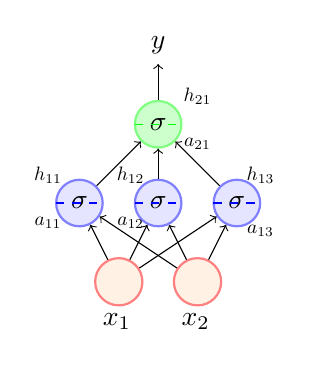
\begin{tikzpicture}
	
	\node [input_neuron] (in1) at (6.5,1)  {} ;
	\node [input_neuron] (in2) at (7.5,1)  {} ;
	%\node (input1) at (6.5,0)  {$x_{1}$};
	%\node (input2) at (7.5,0)  {$x_{2}$};
	\node (output1) at (7,4)  {$y$};
	\node [hidden_neuron] (h1) at (6,2)  {$\sigma$};
	\node [hidden_neuron] (h2) at (7,2)  {$\sigma$};
	\node [hidden_neuron] (h3) at (8,2)  {$\sigma$};
	\node [output_neuron] (o1) at (7,3)  {$\sigma$};
	
	\node[text width=0.005cm] at (6.3,0.5) {$x_{1}$};
	\node[text width=0.005cm] at (7.3,0.5) {$x_{2}$};
	
	%\draw [->] (input1) -- (in1);
	%\draw [->] (input2) -- (in2);
	
	\draw [->] (in1) -- (h1);
	\draw [->] (in1) -- (h2);
	\draw [->] (in1) -- (h3);
	\draw [->] (in2) -- (h1);
	\draw [->] (in2) -- (h2);
	\draw [->] (in2) -- (h3);
	
	\draw [->] (h1) -- (o1);
	\draw [->] (h2) -- (o1);
	\draw [->] (h3) -- (o1);
	
	\draw [->] (o1) -- (output1);
	
	\draw[green,dashed] (6.7,3) -- (7.3,3);
	\draw[blue,dashed] (5.7,2) -- (6.3,2);
	\draw[blue,dashed] (6.7,2) -- (7.3,2);
	\draw[blue,dashed] (7.7,2) -- (8.3,2);
	
	\node (formula)[scale=.7] at (7.5,3.35) {$h_{21}$};
	\node (formula)[scale=.7] at (7.5,2.75) {$a_{21}$};
	
	\node (formula)[scale=.7] at (5.6,2.35) {$h_{11}$};
	\node (formula)[scale=.7] at (6.65,2.35) {$h_{12}$};
	\node (formula)[scale=.7] at (8.3,2.35) {$h_{13}$};
	
	\node (formula)[scale=.7] at (5.6,1.75) {$a_{11}$};
	\node (formula)[scale=.7] at (6.65,1.75) {$a_{12}$};
	\node (formula)[scale=.7] at (8.3,1.65) {$a_{13}$};
	
\end{tikzpicture}